\documentclass[10pt,aspectratio=43]{beamer}

\usepackage{tikz}
\usepackage{xcolor}
\usepackage{caption}
\usepackage{subcaption}
\usepackage{bm}
\usetikzlibrary{calc} 
\usepackage{hyperref}
\hypersetup{
    colorlinks=true,
    linkcolor=blue,
    urlcolor=red
}
\usepackage{fontawesome5}
\usepackage{ulem}

\usetheme{MyStyle}   % loads beamerthemeMyStyle.sty
\setlength{\columnsep}{0pt}


%%%%%%%%%%%%%%%%%%%%%%%%%%%%%%%%%%%%%%%%%%
%%%%%%%%%%%%%%%%%%%%%%%%%%%%%%%%%%%%%%%%%%
%%%%%%%%%%%%%%%%%%%%%%%%%%%%%%%%%%%%%%%%%%

\title{AHDC alignment}
\newcommand{\eventname}{ALERT meeting}
\author{Felix Touchte Codjo}
\institute{IJCLab}
\date{\today}


\begin{document}

\begin{frame}[plain] % remove header, footer, barre de navigation
\titlepage
\end{frame}

%\begin{frame}{Outline}
%\tableofcontents
%\end{frame}

%\section{Intro}
\section{Updates}
\begin{frame}{Updates - wire alignment}
    % \begin{itemize}
    %     \item I started the alignment of the wires, but I faced some issue...
    %     \item 
    % \end{itemize}
    
    % \vspace{0.2cm}
    % \centering
    \begin{minipage}{0.36\textwidth}
        \begin{itemize}
            \item I started the alignment of the wires, but I faced some issue...
            \item On the right, we have the residual LR distribution for some wires (belonging to fitted tracks)
            \item Some of them are well centered (it comes from the previous layer alignment)
            \item Others are weird.
            \item At the beginning, we noticed that they usually appear by pair.
            \item They may have been switched.
        \end{itemize}
    \end{minipage}
    \begin{minipage}{0.6\textwidth}
        %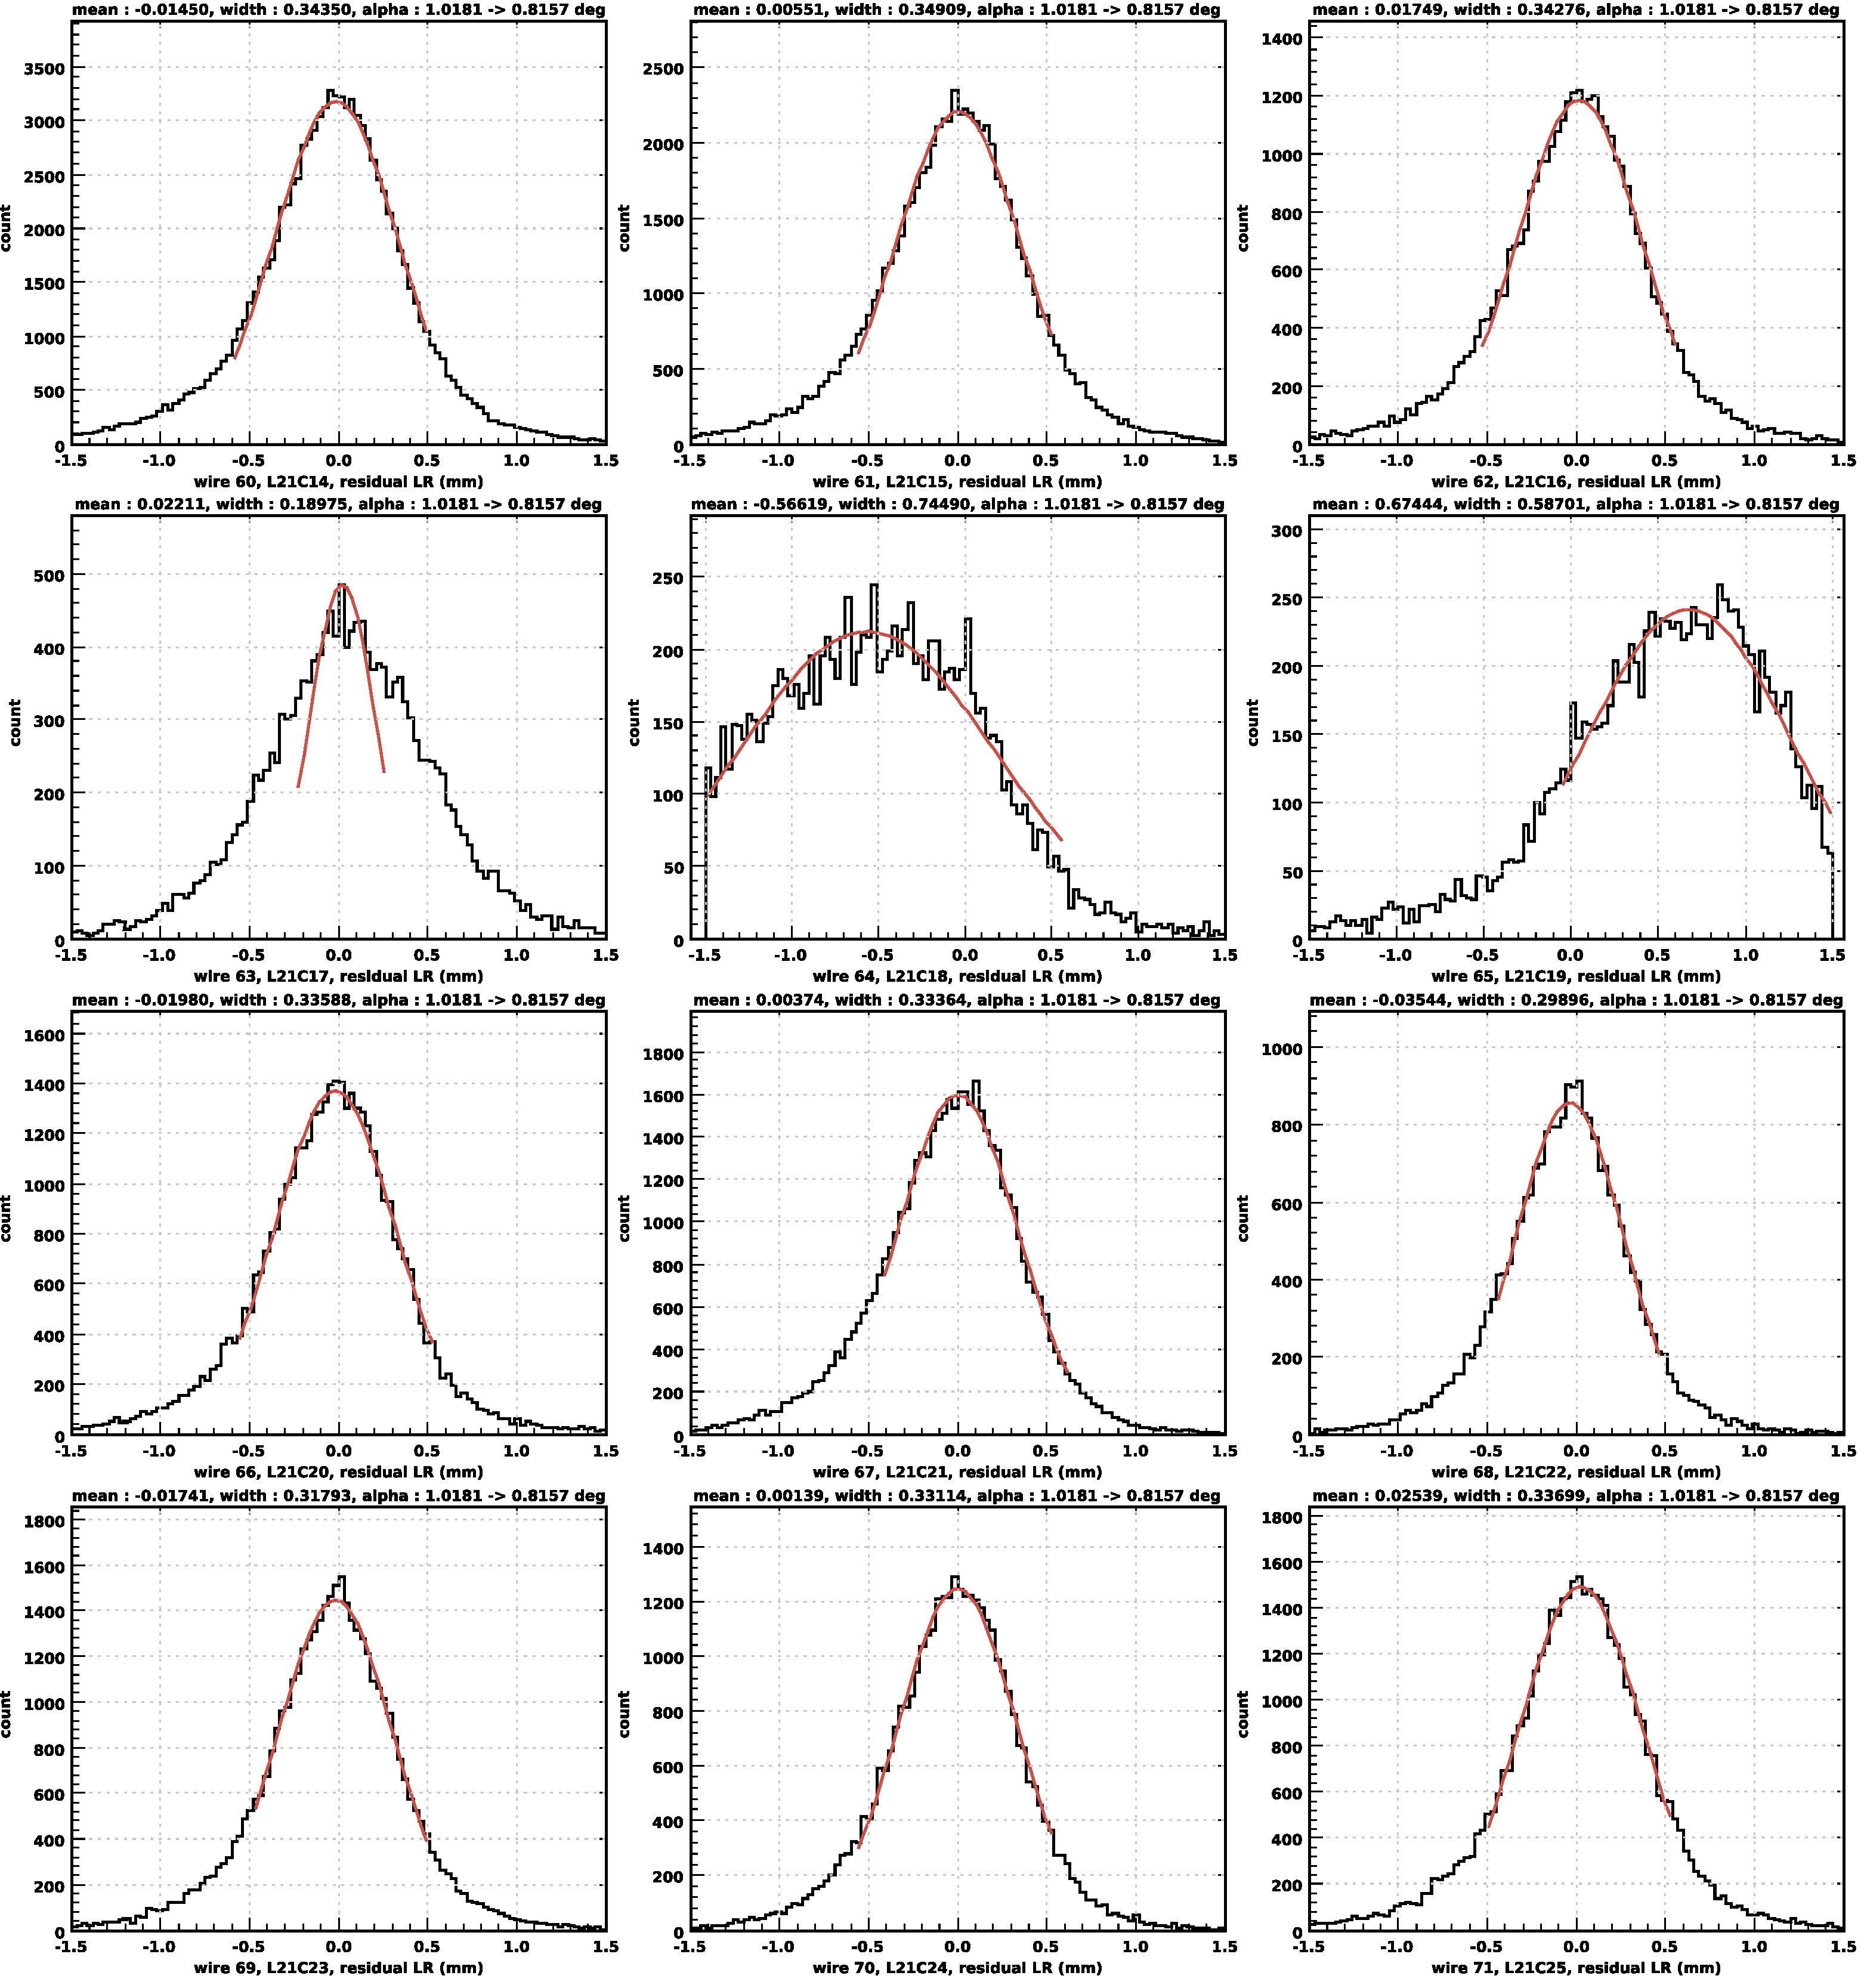
\includegraphics[width=\linewidth]{figures/resilual_LR_iter_1_w60-71.pdf}
        \begin{tikzpicture}
            \node[anchor=south west, inner sep=0] (img) at (0,0)
                {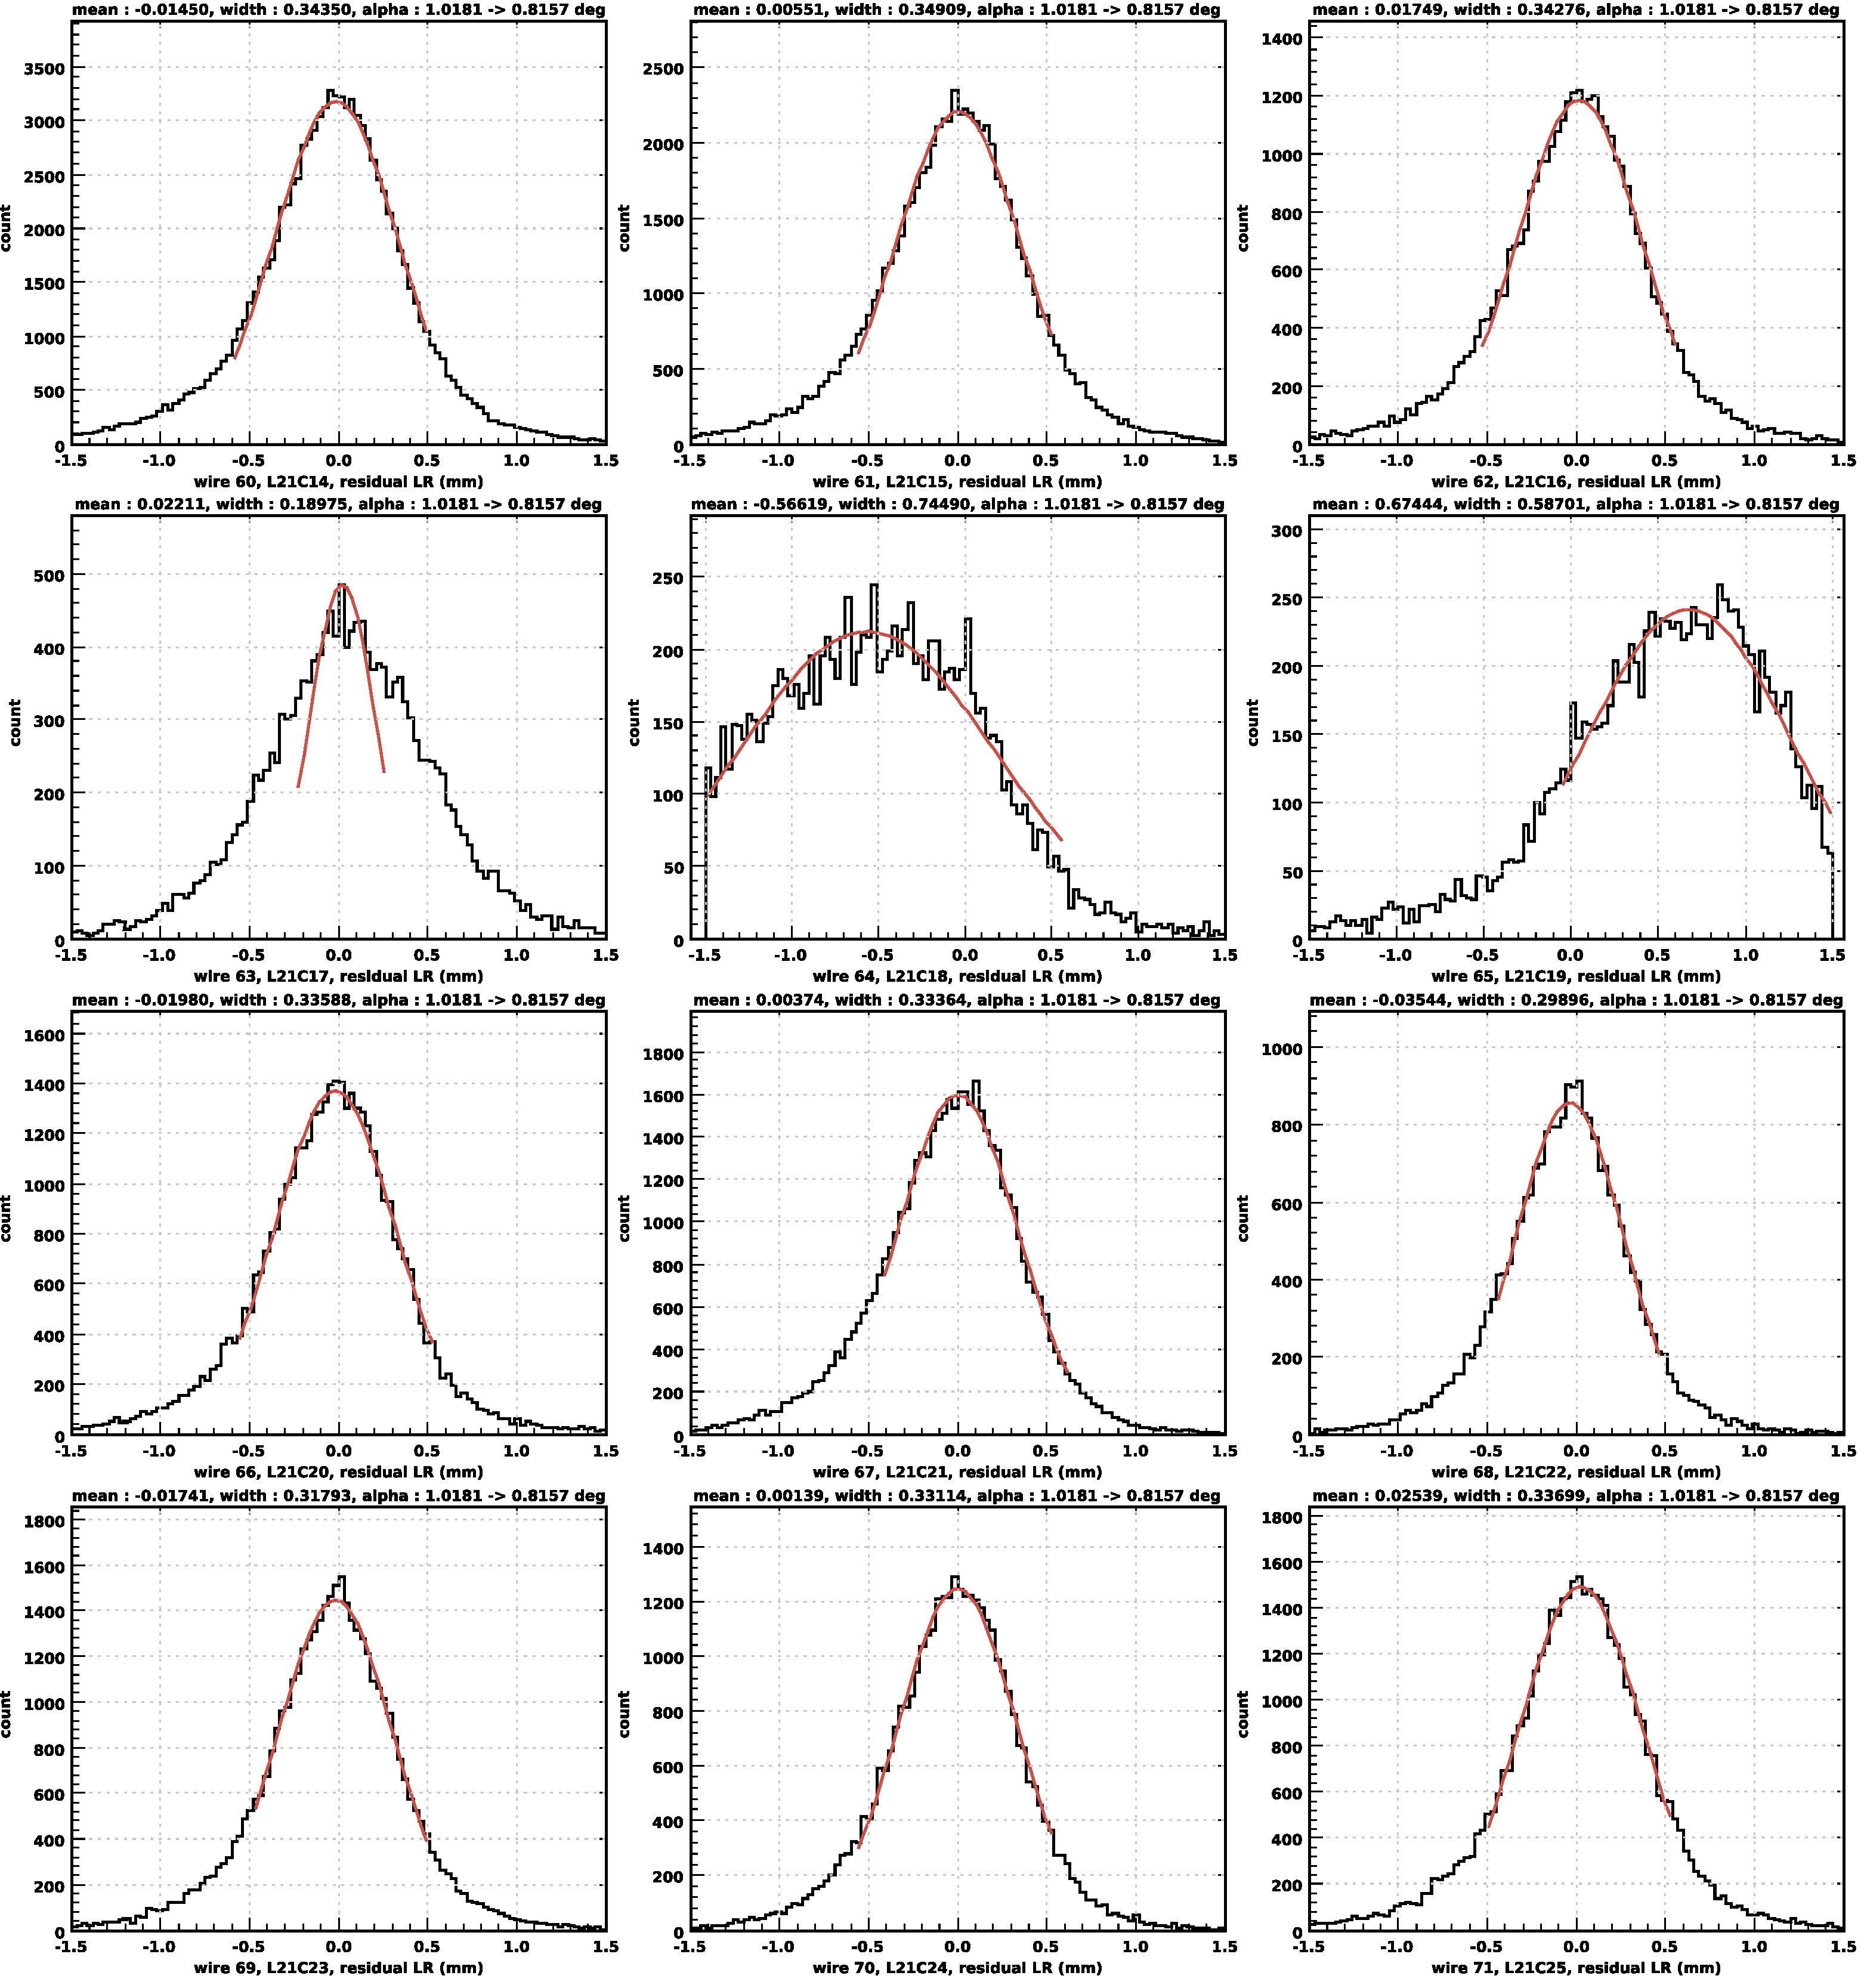
\includegraphics[width=\linewidth]{figures/resilual_LR_iter_1_w60-71.pdf}};
            
            % système de coordonnées normalisé
            \begin{scope}[x={(img.south east)}, y={(img.north west)}]
                % annotation texte
                \node [blue] at (0.58,0.66) {\small 1};
                \node [blue] at (0.8,0.66) {\small 2};
                
                % flèche
                %\draw[->, red, thick] (0.3,0.3) -- (0.5,0.5);
            \end{scope}
        \end{tikzpicture}

    \end{minipage}
    
\end{frame}

\begin{frame}{Updates - wire alignment}
    % \begin{itemize}
    %     \item I started the alignment of the wires, but I faced some issue...
    %     \item 
    % \end{itemize}
    
    % \vspace{0.2cm}
    % \centering
    \begin{minipage}{0.36\textwidth}
        \begin{itemize}
            \item I started the alignment of the wires, but I faced some issue...
            \item On the right, we have the residual LR distribution for some wires (belonging to fitted tracks)
            \item Some of them are well centered (it comes from the previous layer alignment)
            \item Others are weird.
            \item At the beginning, we noticed that they usually appear by pair. 
            \item They may have been switched.
        \end{itemize}
    \end{minipage}
    \begin{minipage}{0.6\textwidth}
        %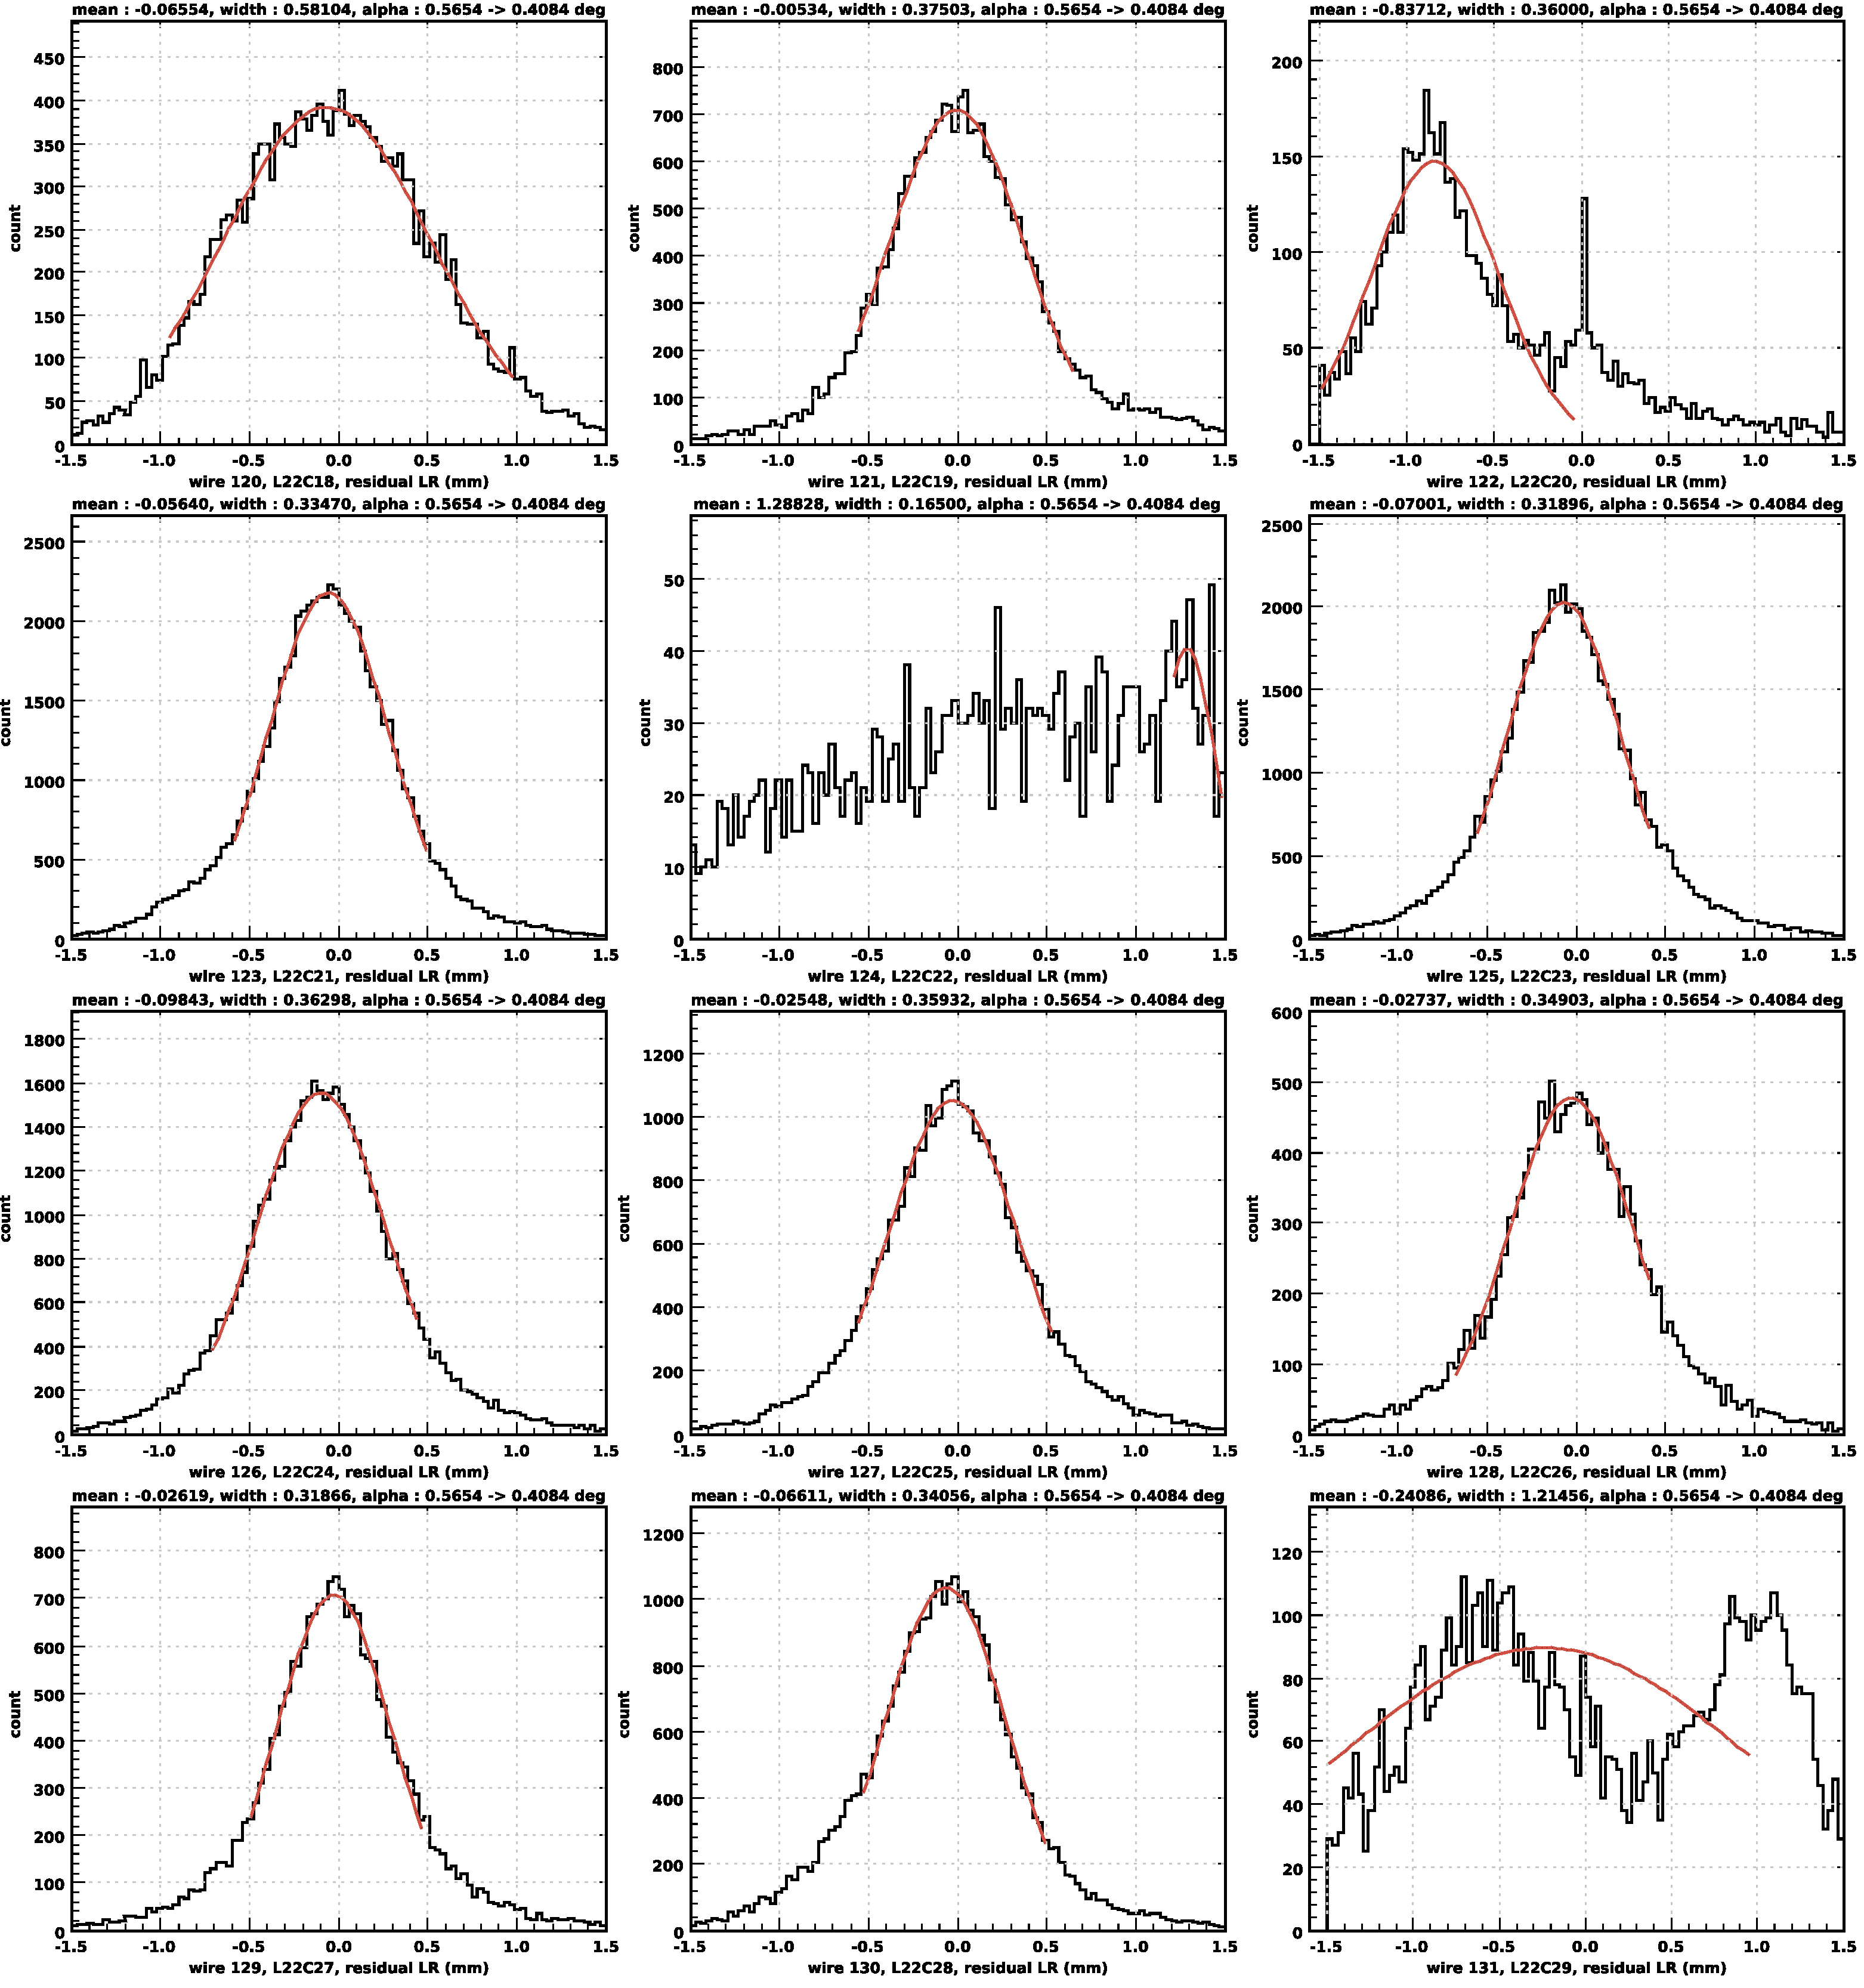
\includegraphics[width=\linewidth]{figures/resilual_LR_iter_1_w120-131.pdf}
        \begin{tikzpicture}
            \node[anchor=south west, inner sep=0] (img) at (0,0)
                {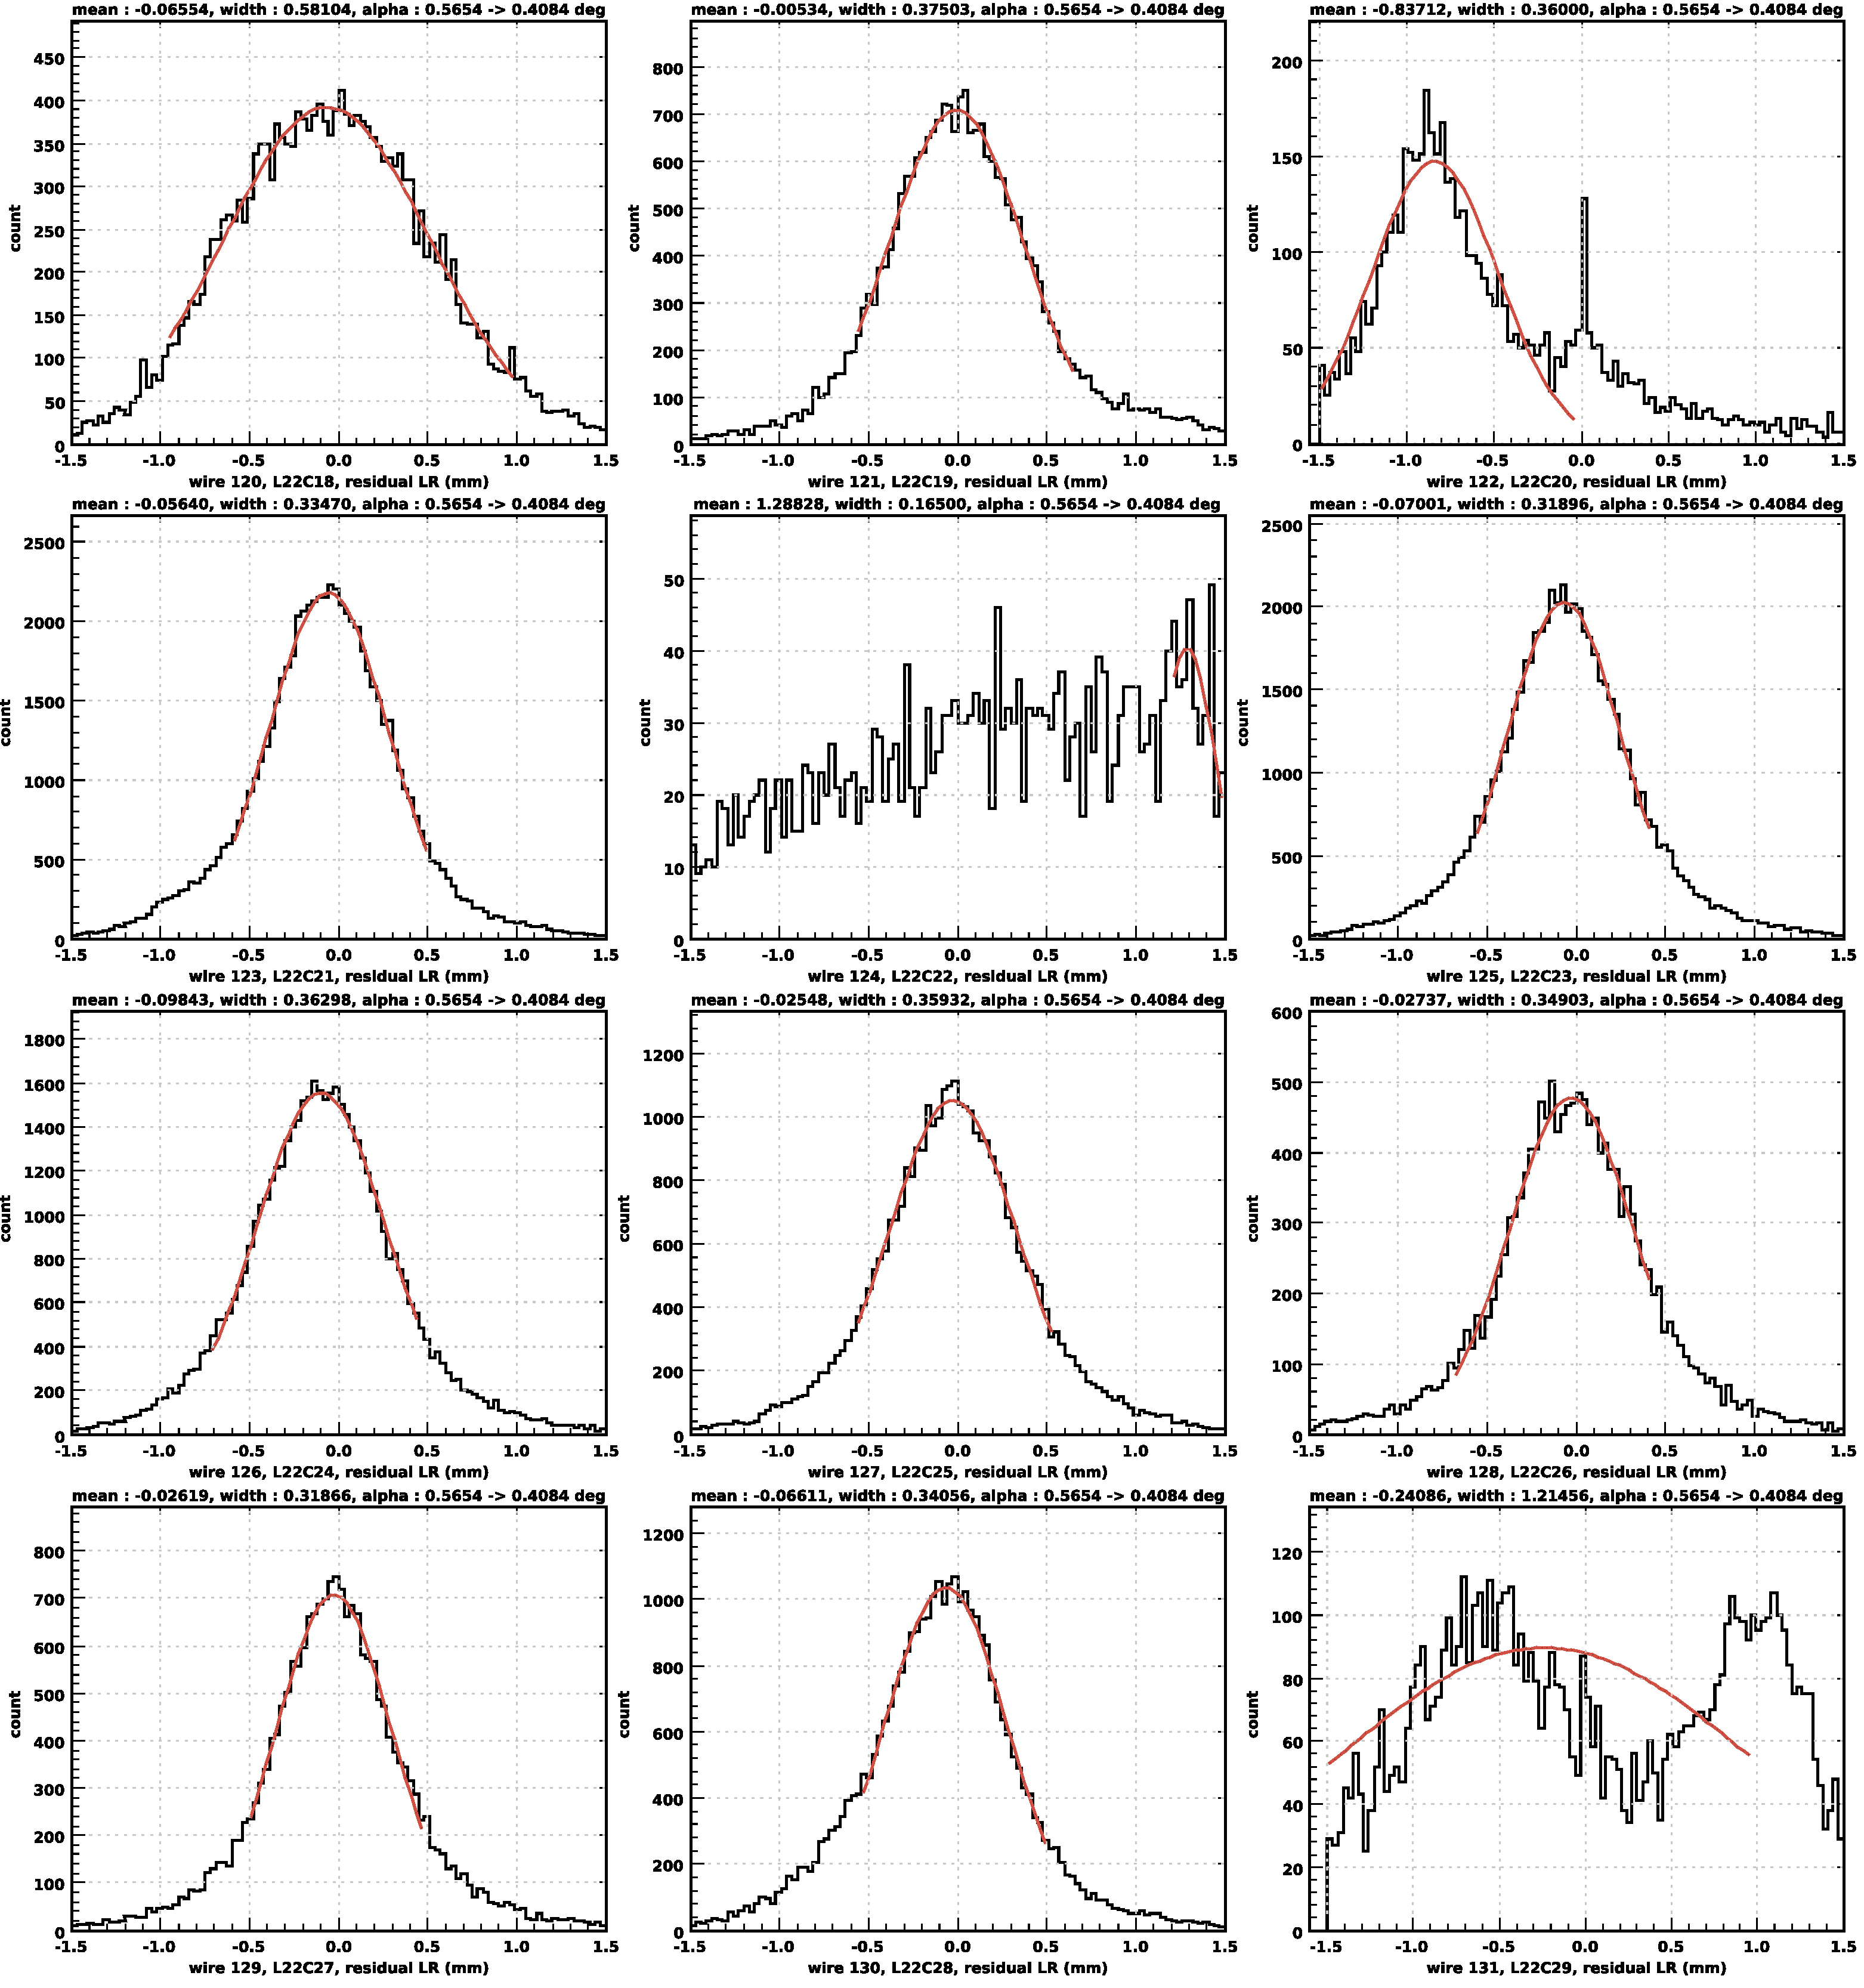
\includegraphics[width=\linewidth]{figures/resilual_LR_iter_1_w120-131.pdf}};
            
            % système de coordonnées normalisé
            \begin{scope}[x={(img.south east)}, y={(img.north west)}]
                % annotation texte
                \node [blue] at (0.58,0.7) {\small 2};
                \node [blue] at (0.9,0.90) {\small 1};
                
                % flèche
                %\draw[->, red, thick] (0.3,0.3) -- (0.5,0.5);
            \end{scope}
        \end{tikzpicture}
    \end{minipage}
    
\end{frame}

\begin{frame}{Updates - wire alignment}
    \begin{itemize}
        \item We decided to look at the wire disposition per layer versus the electron's $\phi$
        \item The two red circles match the two set of weird distributions that we saw in the last slides
    \end{itemize}

    \centering

    \begin{tikzpicture}
        \node[anchor=south west, inner sep=0] (img) at (0,0)
            {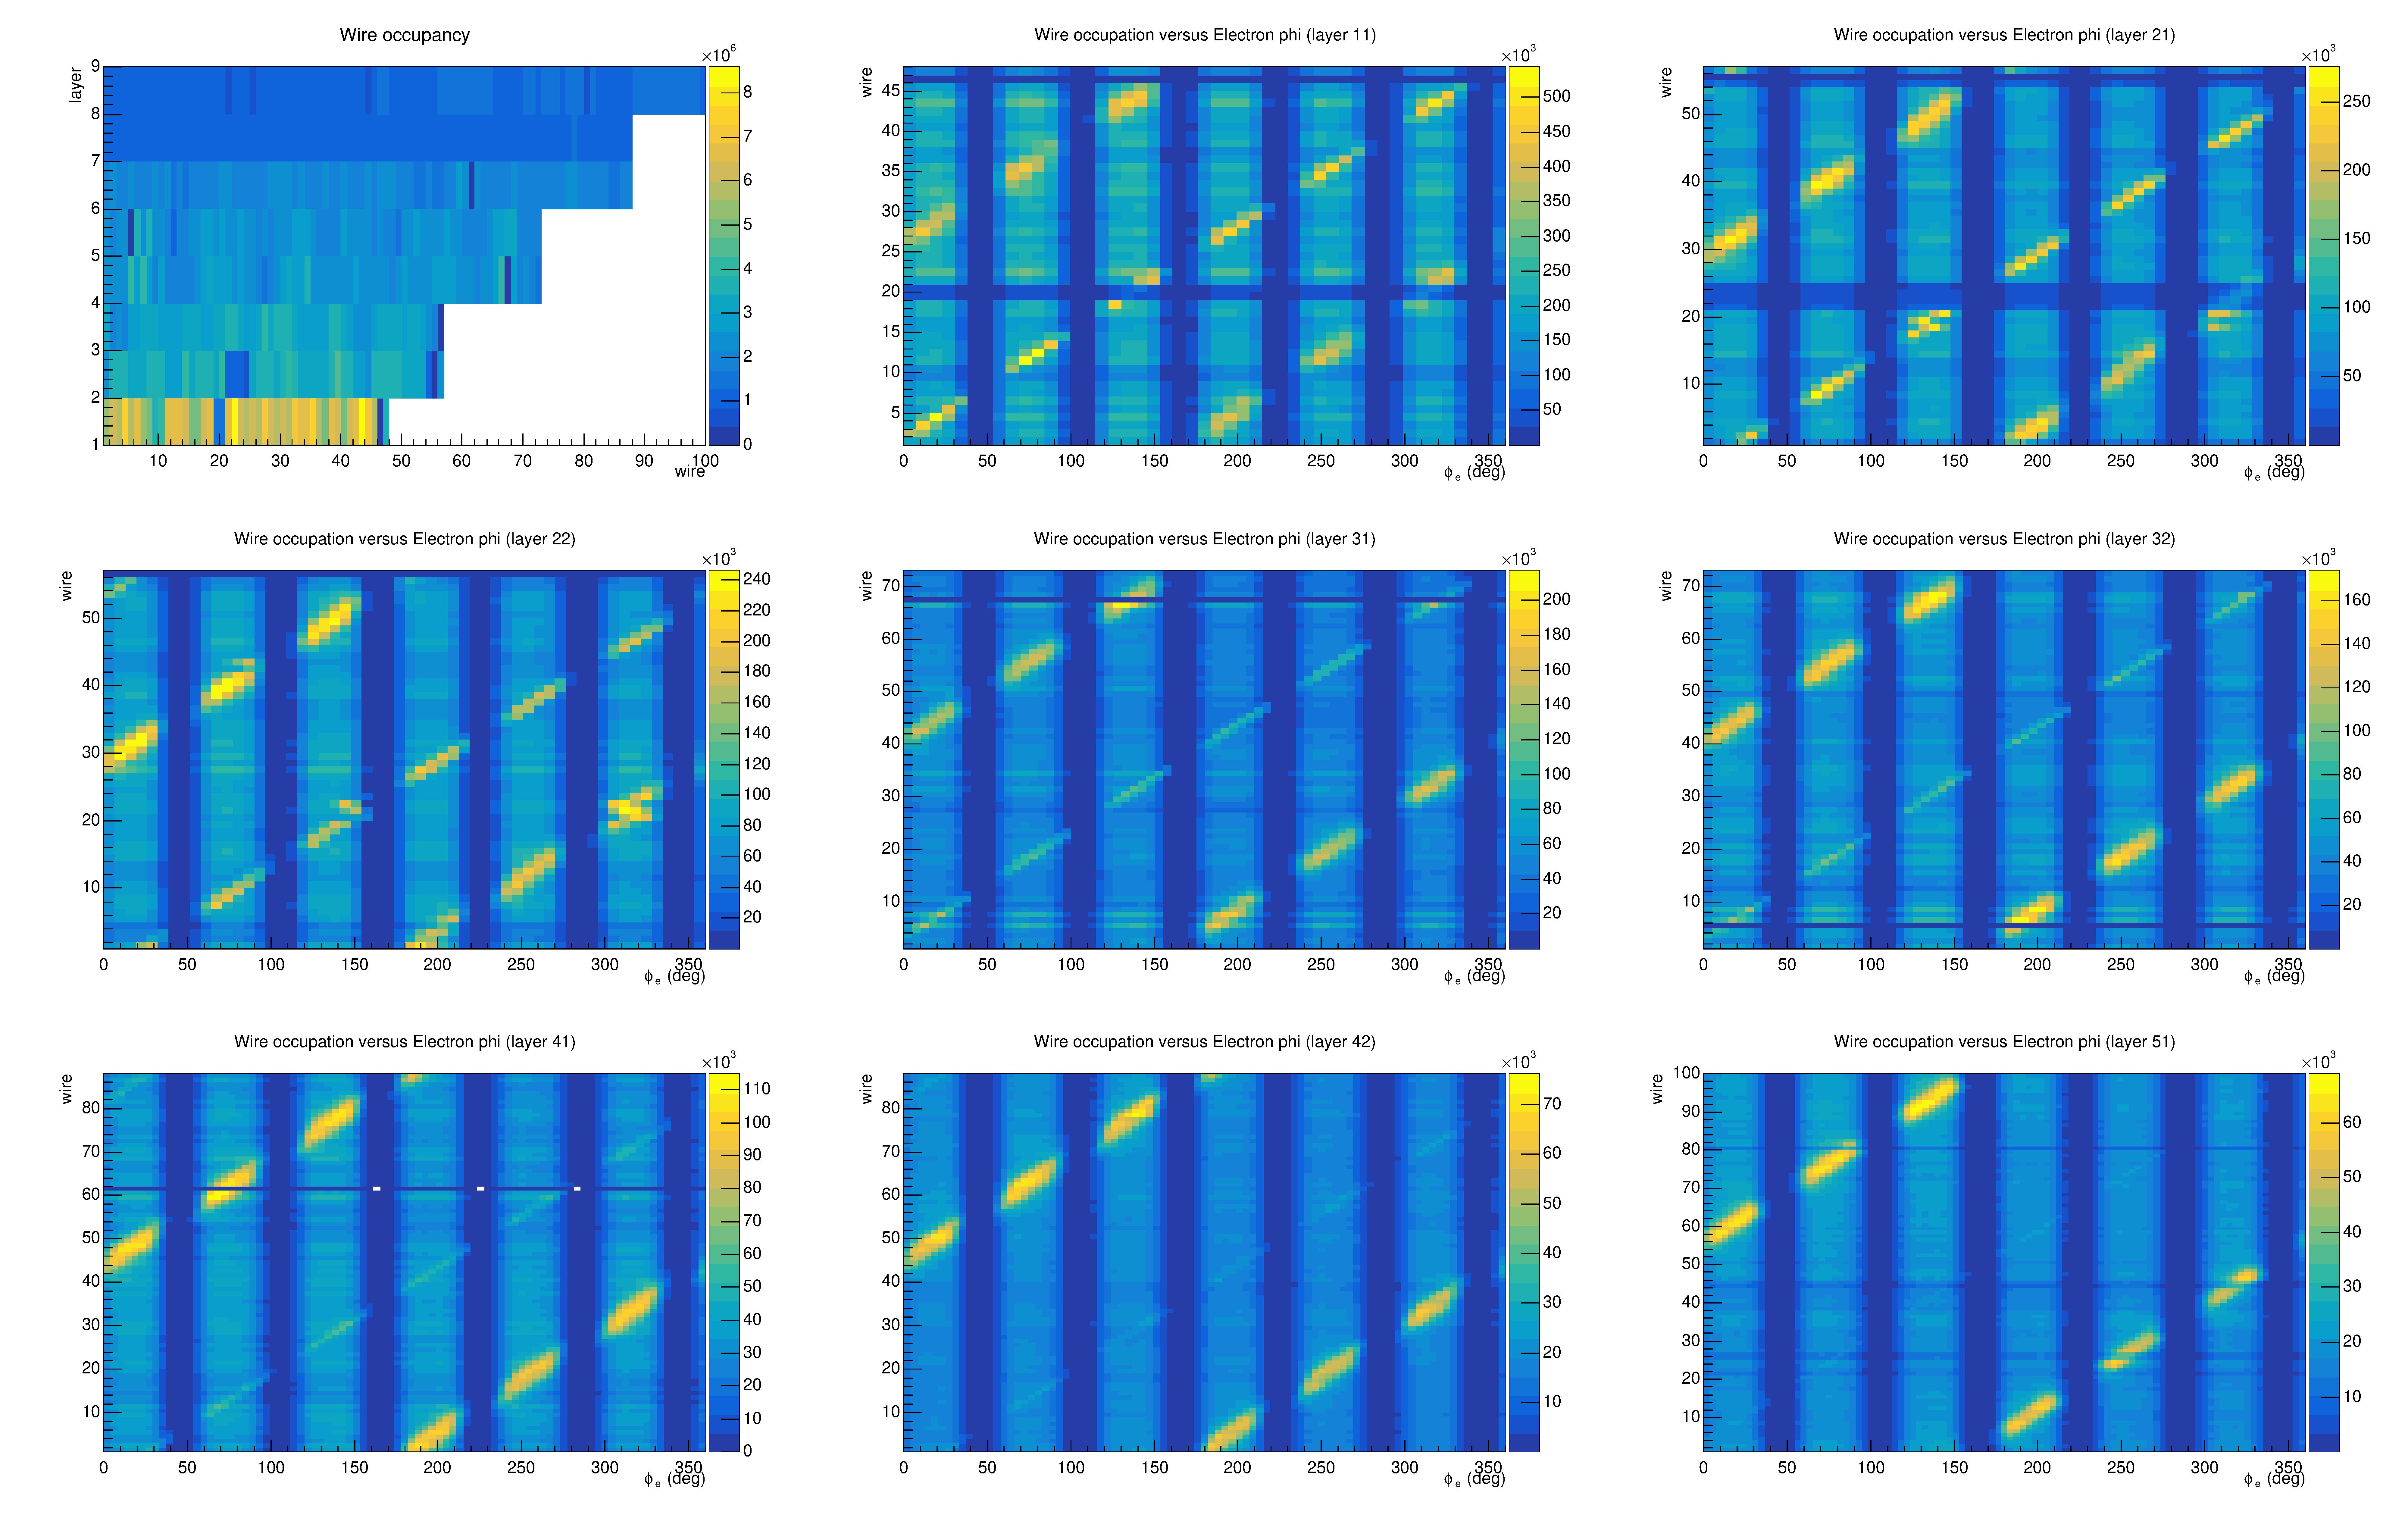
\includegraphics[width=0.9\linewidth]{figures/wire_disposition_vs_electron_phi.pdf}};
        
        % système de coordonnées normalisé
        \begin{scope}[x={(img.south east)}, y={(img.north west)}]
            % annotation texte
            \draw [red] (0.26,	0.47) circle [radius=0.02];
            \draw [red] (0.92,	0.79) circle [radius=0.02];
            
            % flèche
            %\draw[->, red, thick] (0.3,0.3) -- (0.5,0.5);
        \end{scope}
    \end{tikzpicture}

    %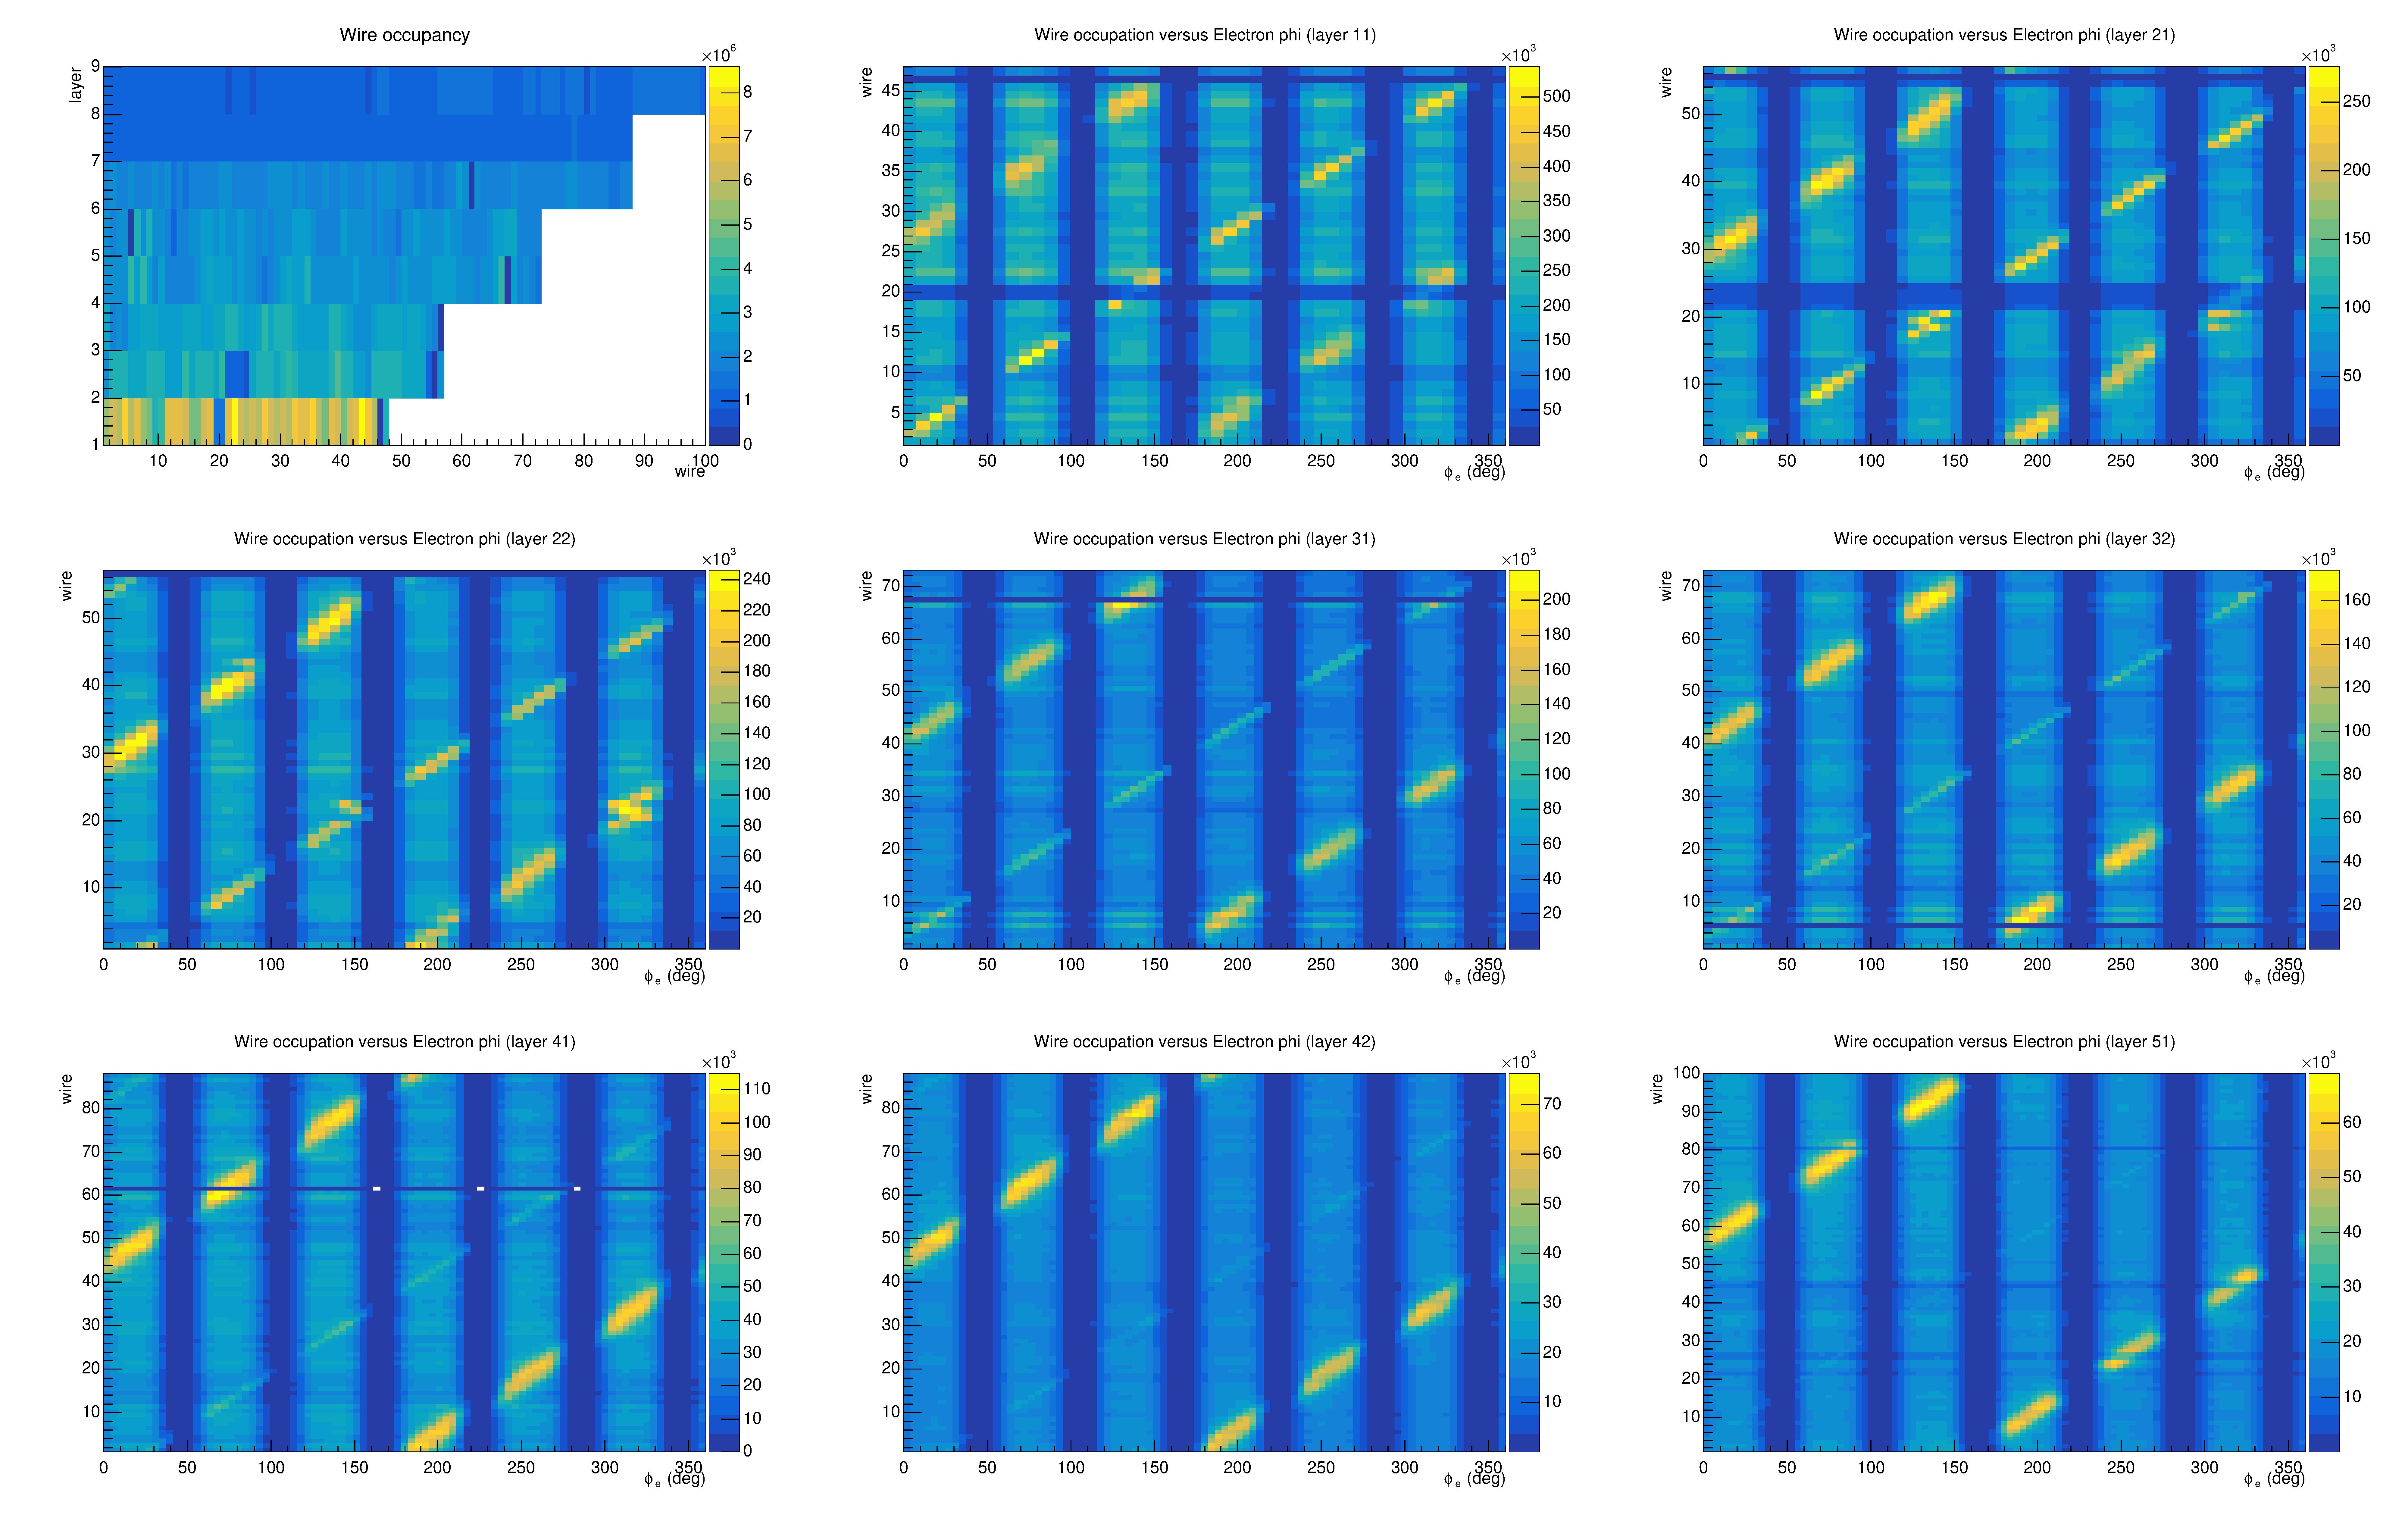
\includegraphics[width=0.85\linewidth]{figures/wire_disposition_vs_electron_phi.pdf}
    
    
\end{frame}

\begin{frame}{Updates - wire alignment}

    \begin{minipage}{0.36\textwidth}
        \begin{itemize}
            \item I have initially listed 29 bad distributions
            \item I have already inverted the wires (L21C18, L21C19) and (L22C20, L22C22). That fixed five of them (the filled blue circles)
            \item 24 are still under investigating (the filled black circles)
            \item They are almost arranged into groups.
            \item It is possible that only one wire exchange degrades the residual distribution of the whole group of bad wires
        \end{itemize}
    \end{minipage}
    \begin{minipage}{0.6\textwidth}
        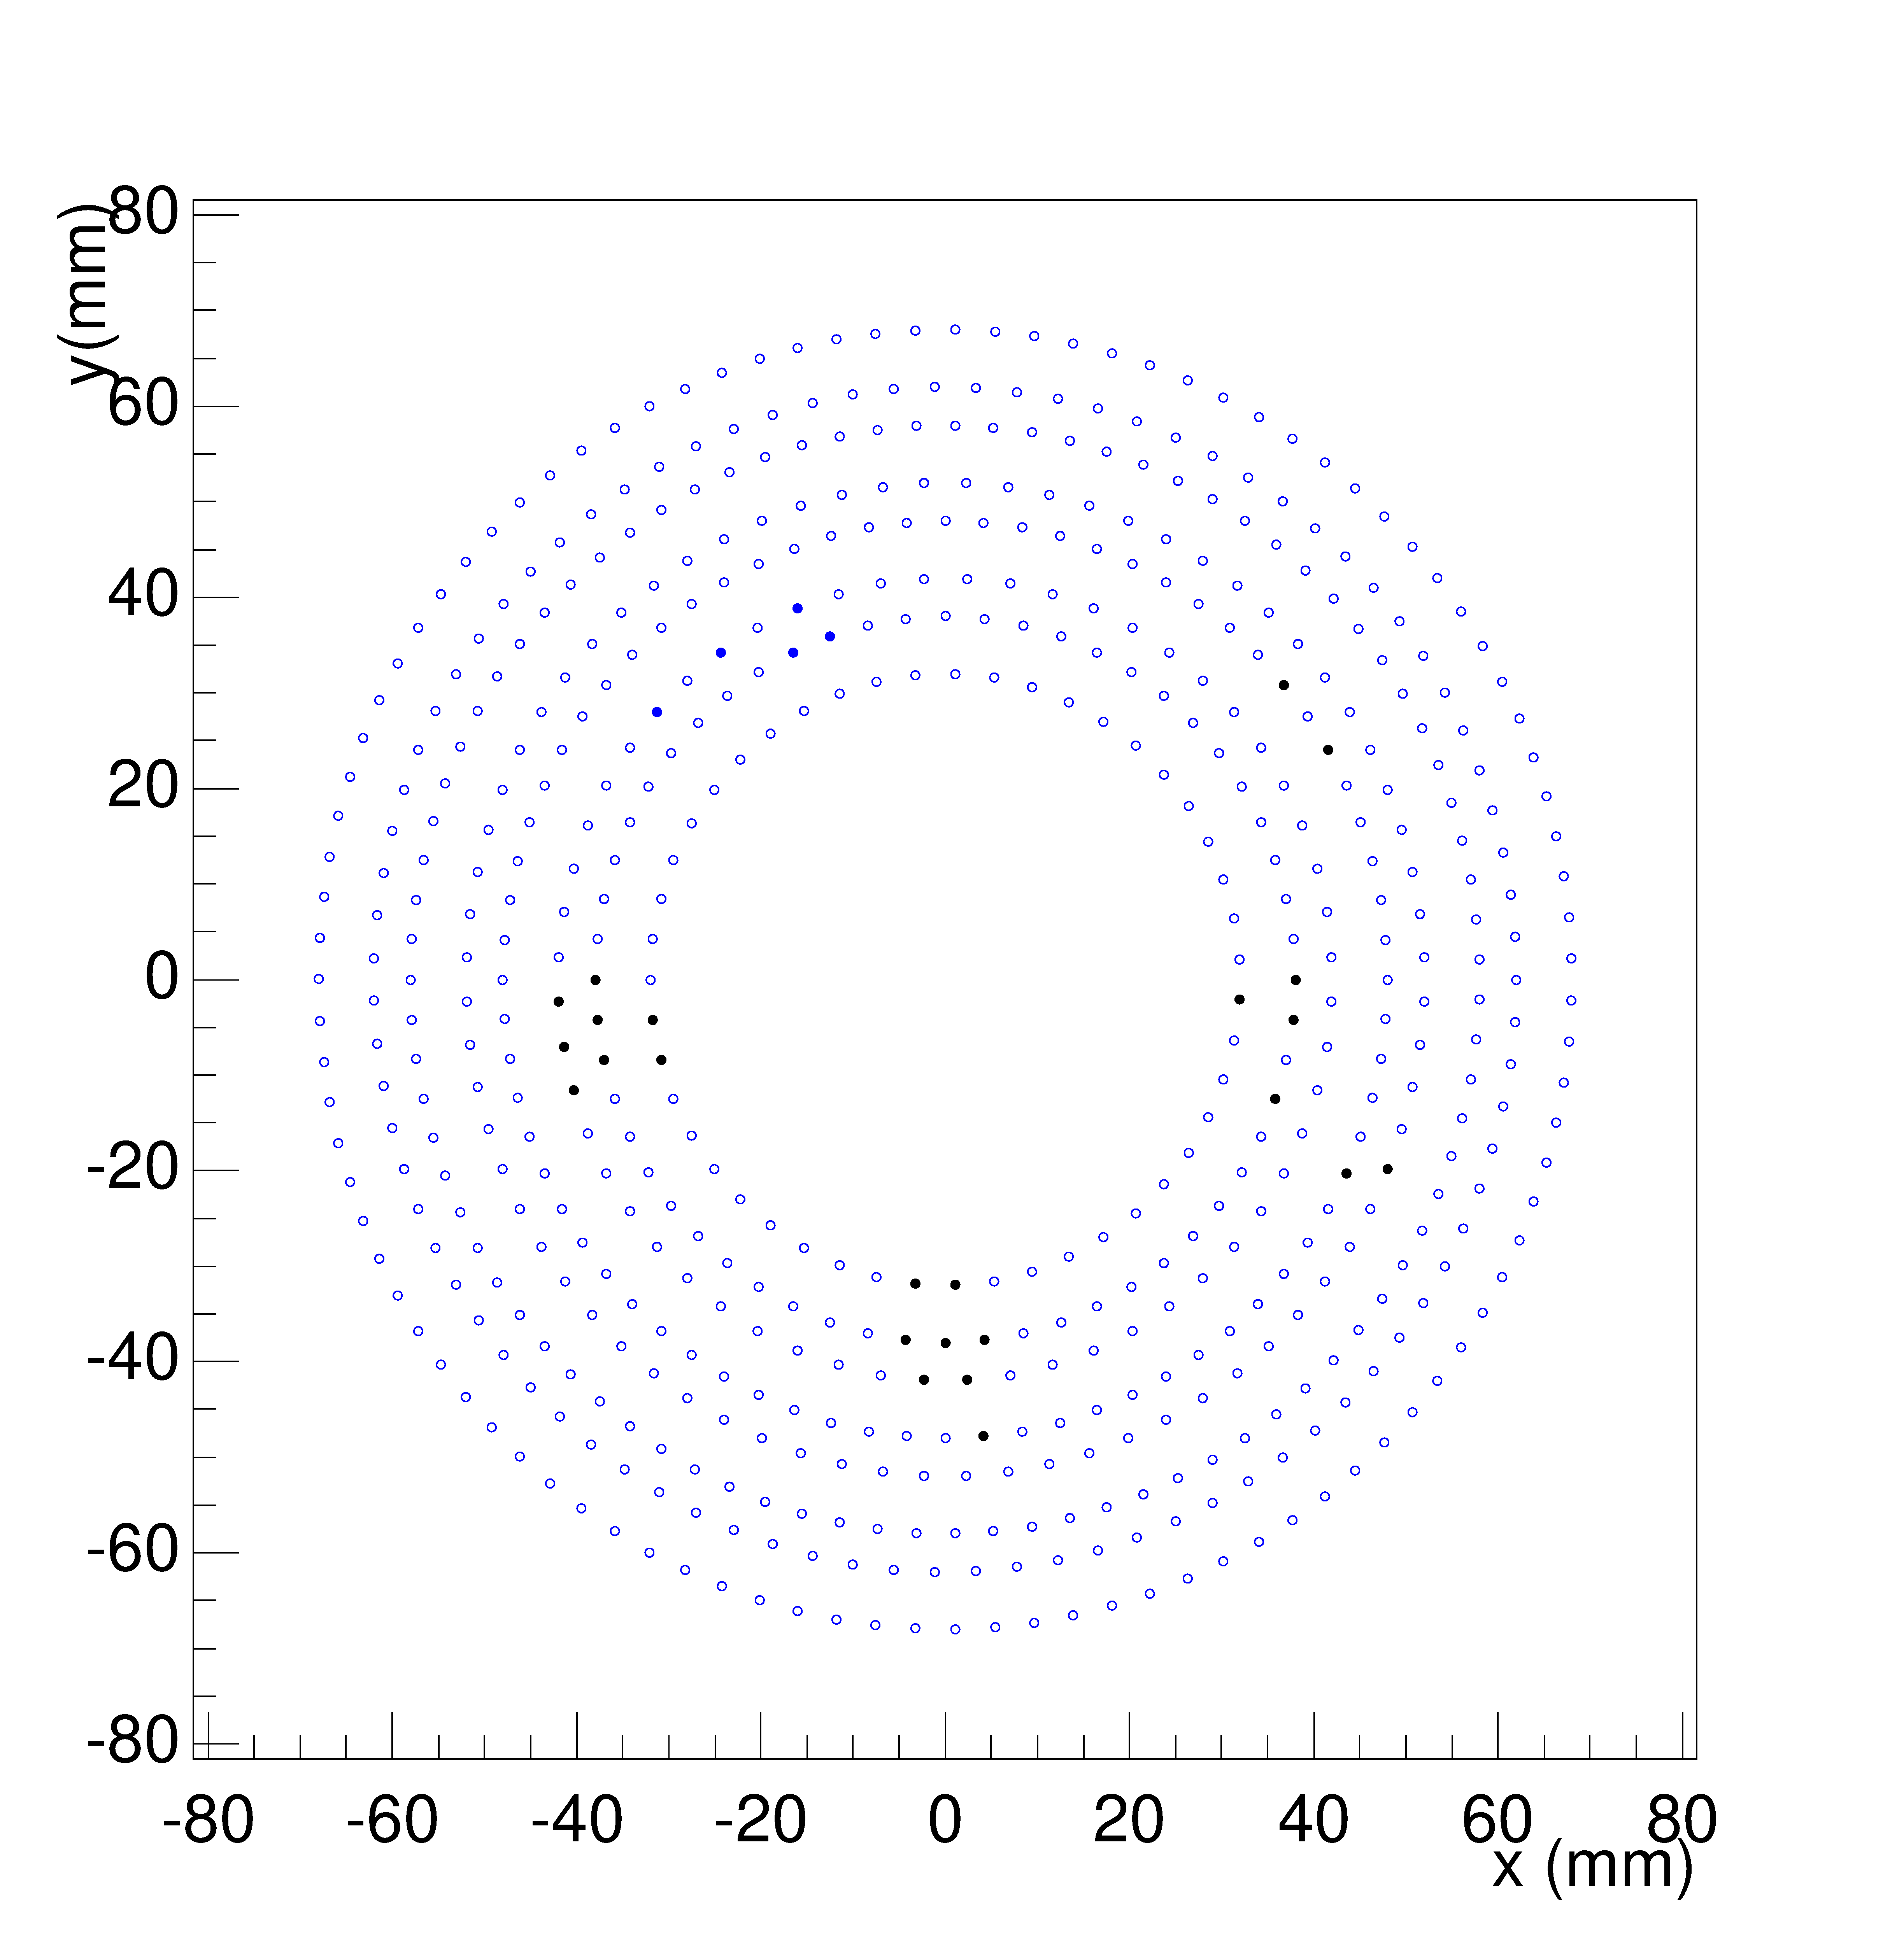
\includegraphics[width=\linewidth]{figures/bad_wires_xyView.pdf}
    \end{minipage}
    

\end{frame}

\begin{frame}{Updates - wire alignment}

    \begin{itemize}
        \item Here are the distribution of the bad wires of the first group
        \item The difficulty here is that we may have some exchanges between wires belonging to different layers. {\color{red} Work in progress...}
    \end{itemize}

    \vspace{0.2cm}
    \centering
    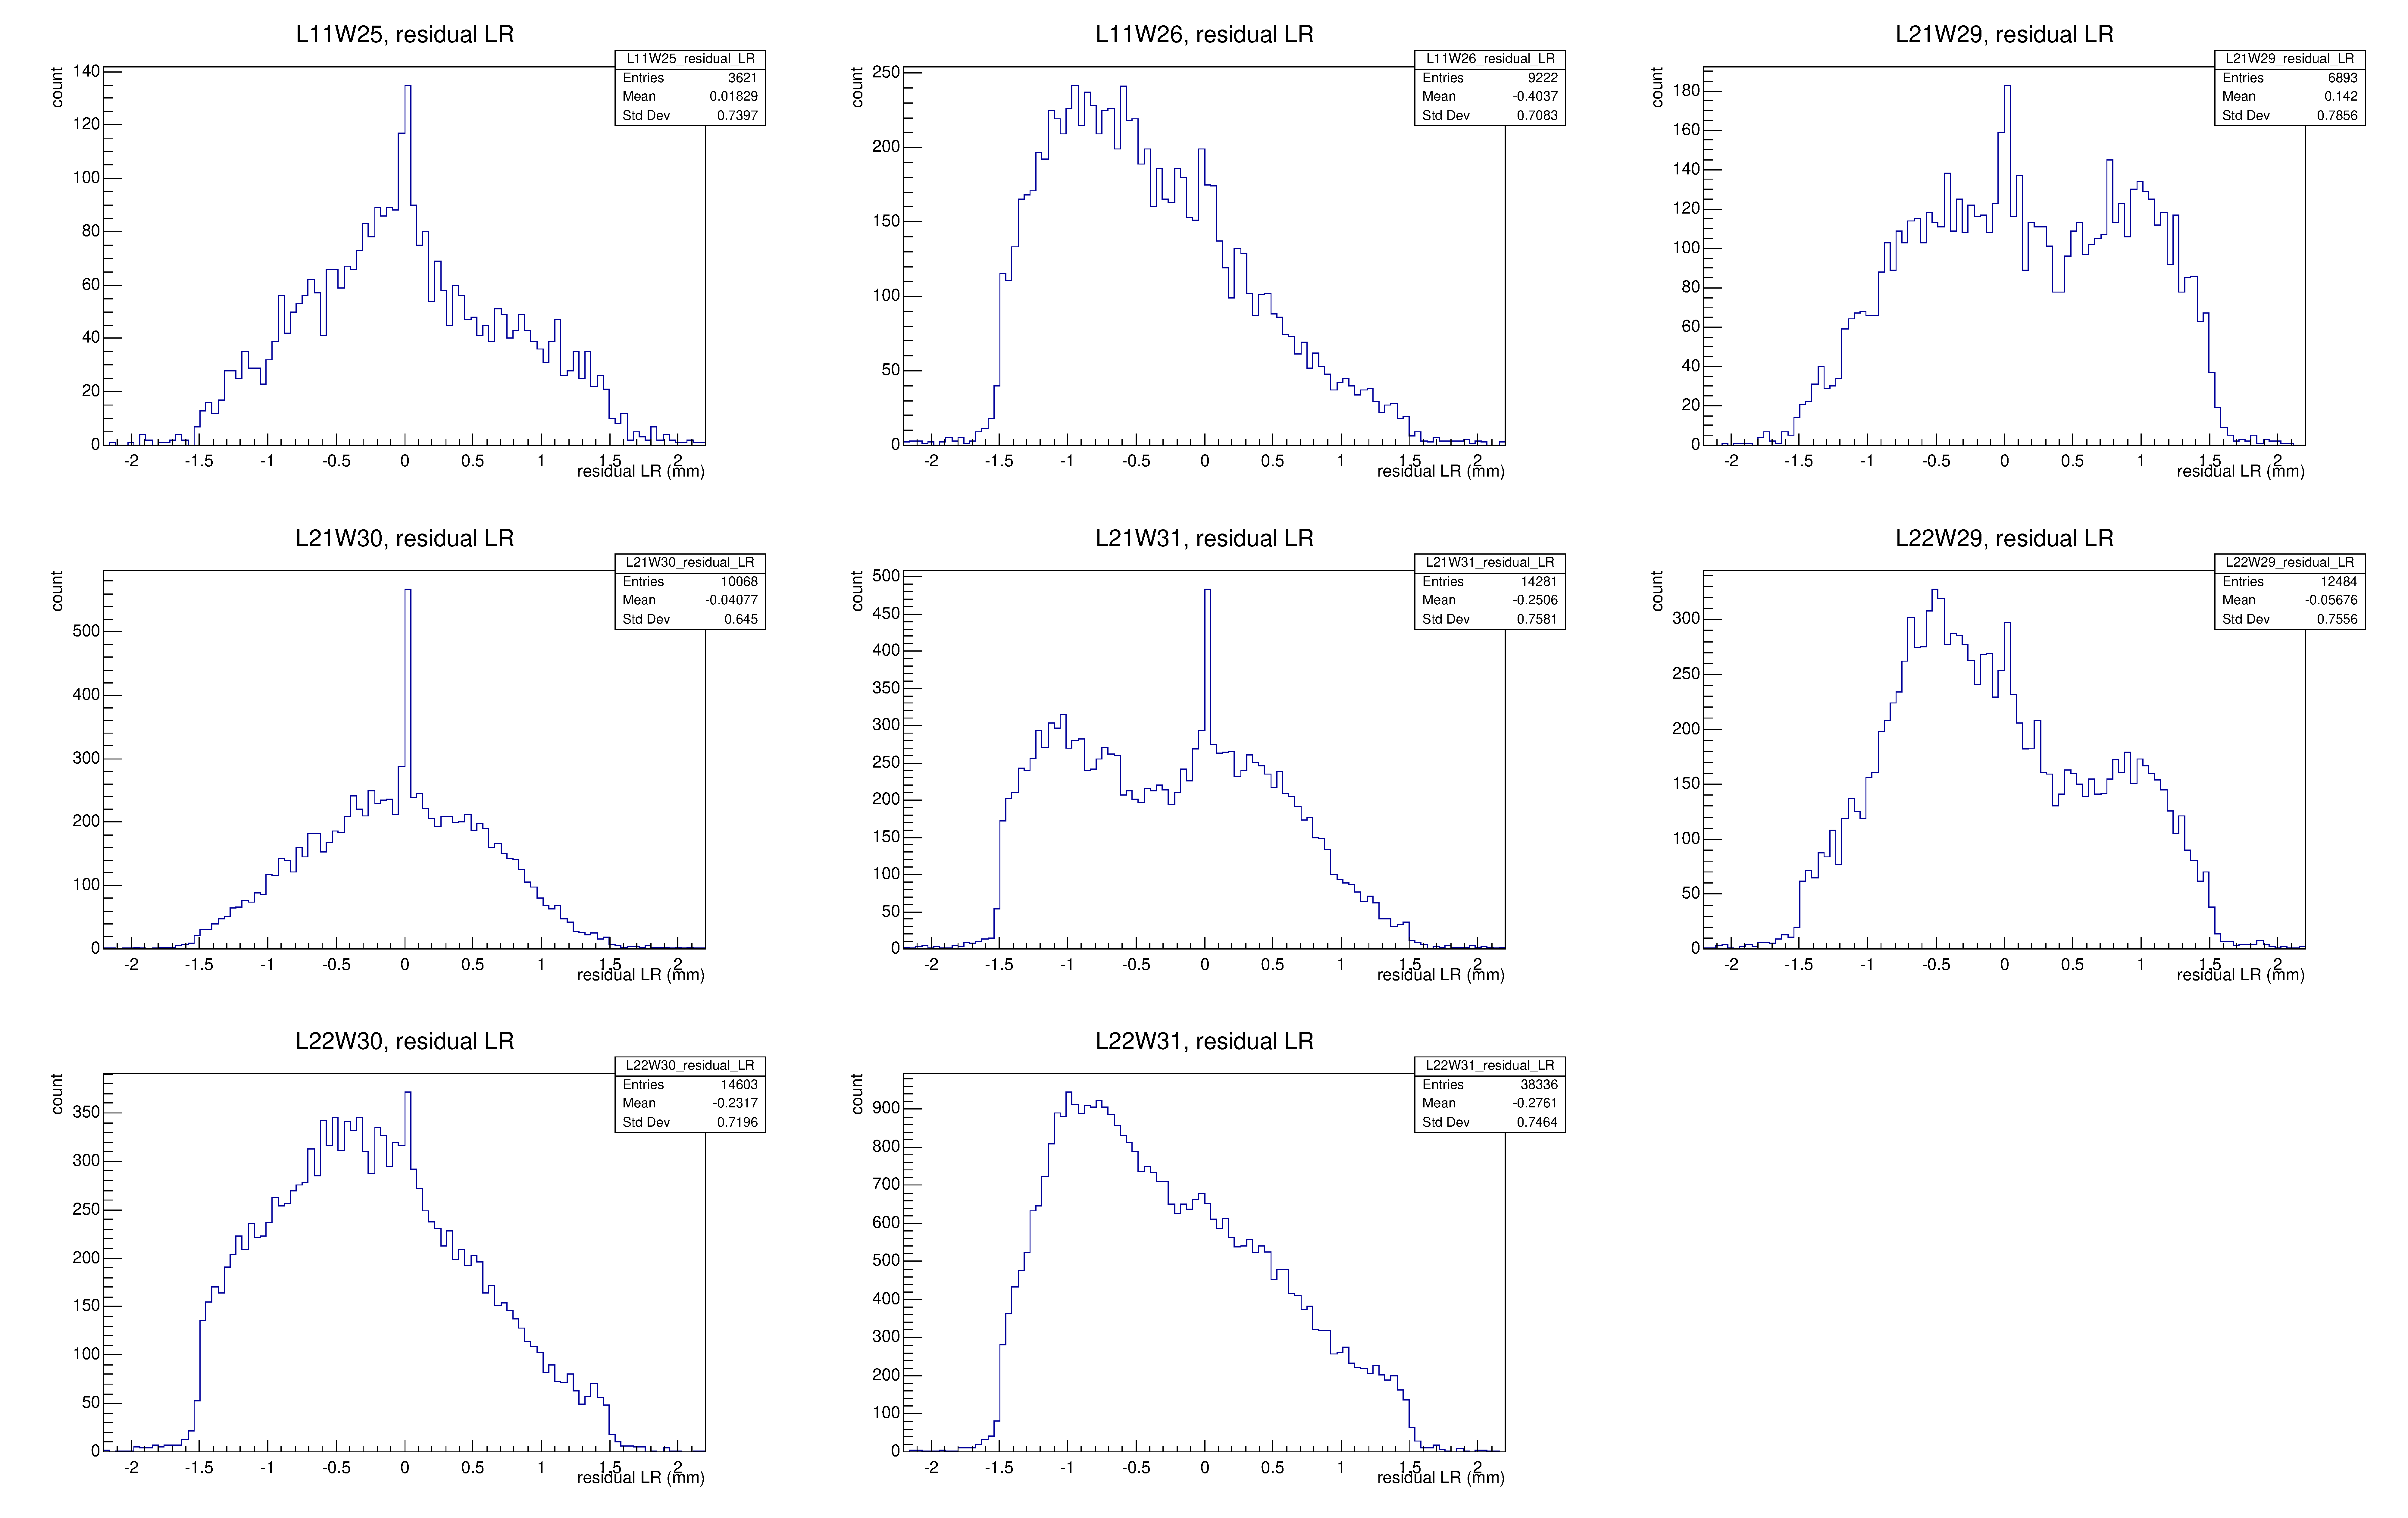
\includegraphics[width=0.85\linewidth]{figures/bad_distributions_group_1.pdf}
    

\end{frame}



% \begin{frame}{Next steps}
%     \begin{itemize}
%         \item I will continue my work on the alignment
%             \begin{itemize}
%                 \item \sout{Rotate independently the two end points of the wires in a given layer}
%                 \item Push the study further by doing a wire by wire alignment
%             \end{itemize}
%         \item Pending task
%             \begin{itemize}
%                 \item Push my work on the ATOF hits for the Kalman Filter in coatjava
%                 \item Finish the work on the Kalman Filter (material verification, target gas density, PID, magnetic field, optimization)
%             \end{itemize}
%     \end{itemize}
    
% \end{frame}



% \begin{frame}{Backup slides}
%     \begin{itemize}
%         \item Procedure:
%             \begin{enumerate}
%                 \item We looked at elastic events : electron + track (here: collection of hits only)
%                 \item We computed the theoretical momentum vector of the track $\vec{p}$
%                 \item We made the propagation without doing any fit (i.e no KF correction)
%                 \item We looked at {\color{blue} residual\_LR} (left-right) $\longrightarrow$ sensitive to the alignment
%             \end{enumerate}
%     \end{itemize}
    

%     \vspace{0.2cm}
%     \centering
%     \begin{minipage}{0.42\textwidth}
%         \includegraphics[width=\linewidth]{figures/build/illustration_residual_type.pdf}
%     \end{minipage}

% \end{frame}






\end{document}


